\section{Concept part}
%From system level specification down to discipline specific
%documentation including diagrams and visualizations \\
%including a comprehensible derivation of your design decisions

\subsection{Szenario}
Der Rescue Roboter wird eingesetzt um Menschen beziehungsweise Lebewesen und Objekte im Fall von Naturkatastrophen oder schweren Unfällen zu retten.
\begin{figure}[htbp] 
  \centering
     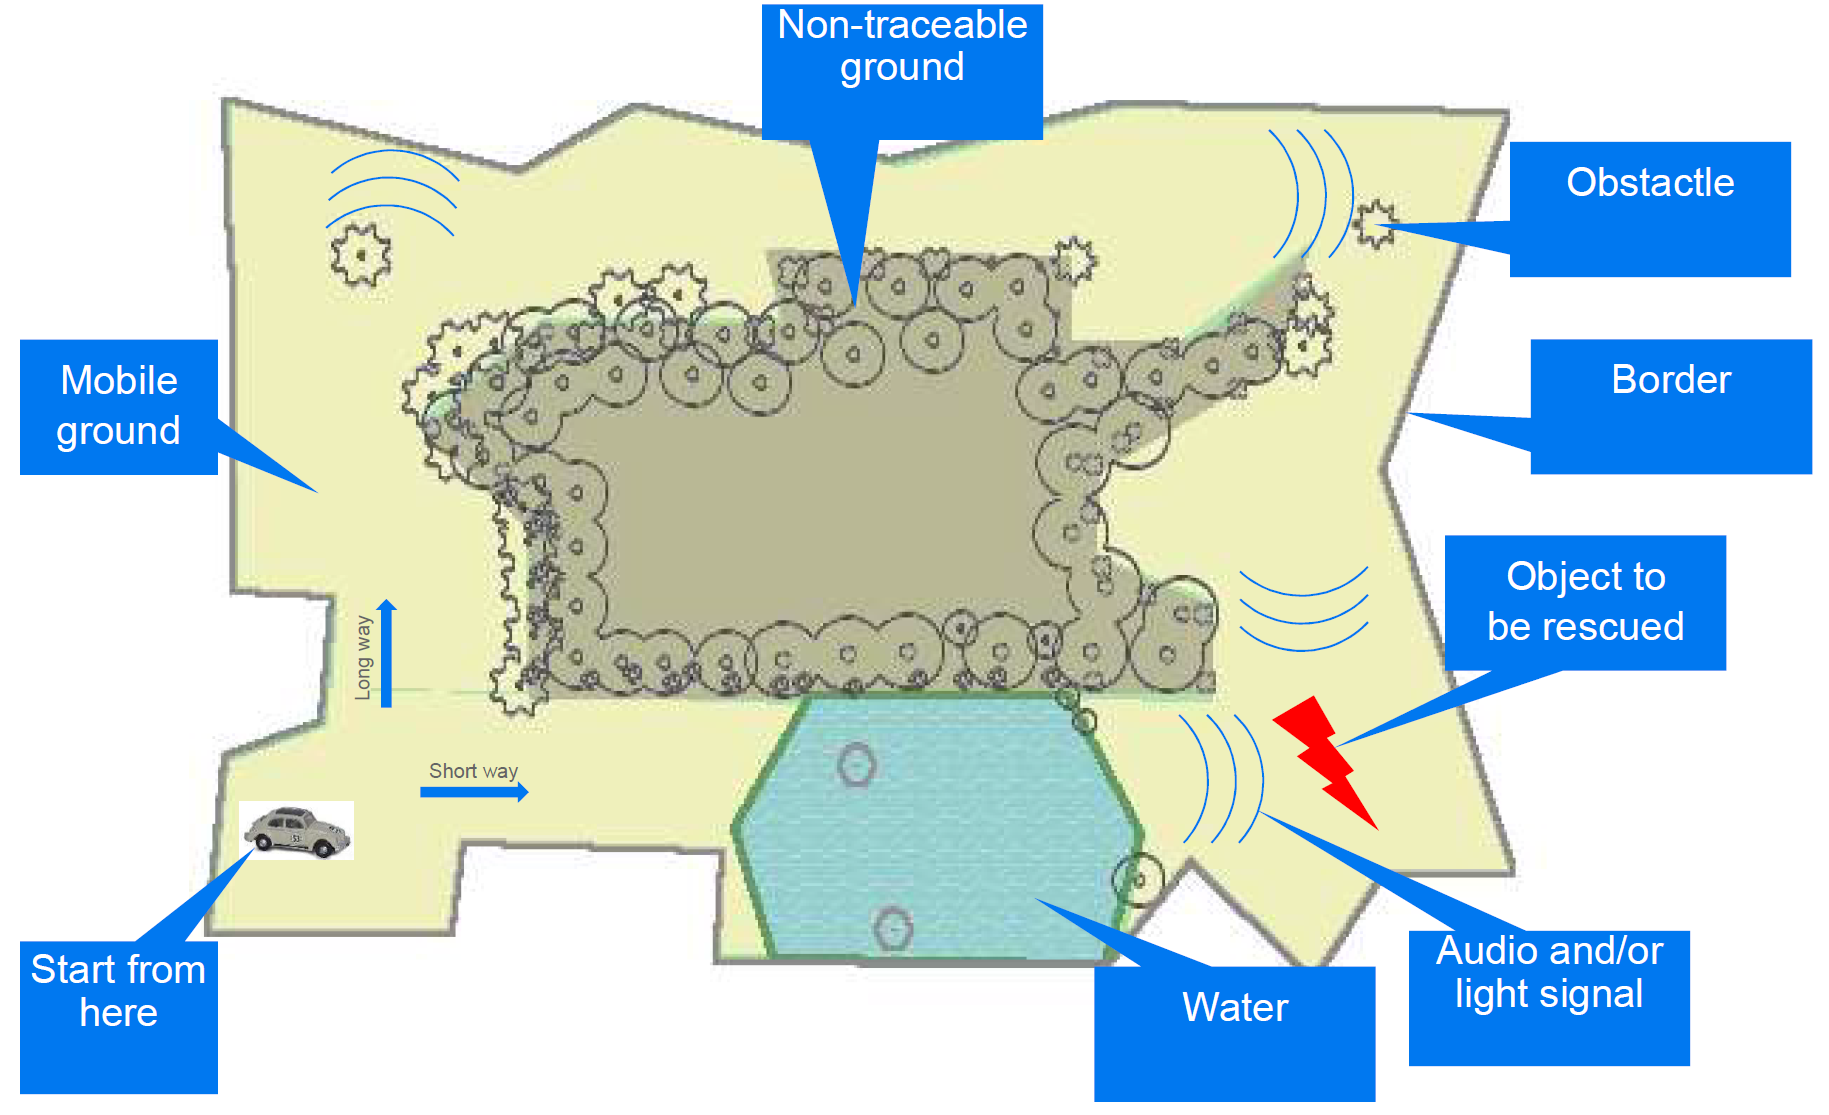
\includegraphics[width=0.5\textwidth]{Bilder/testumgebung.PNG}
  \caption{Testumgebung}
  \label{fig:testumgebung}
\end{figure}\\
Auf der Figur \ref{fig:testumgebung} ist die Testumgebung zu sehen. In diesem Projekt hat der Rescue Roboter die Aufgabe jemanden nach einer Explosion im Mehrfamilienhaus (Figur \ref{fig:testumgebung} "Non-traceable ground") zu bergen. Außerhalb des Hauses finden sich brennende Gegenstände (Figur \ref{fig:testumgebung} "Obstractle") von dem Haus.

\subsection{Anforderungen}
Figur \ref{fig:anforderungen} zeigt die Anforderungen des Projektes.
\begin{figure}[htbp] 
  \centering
     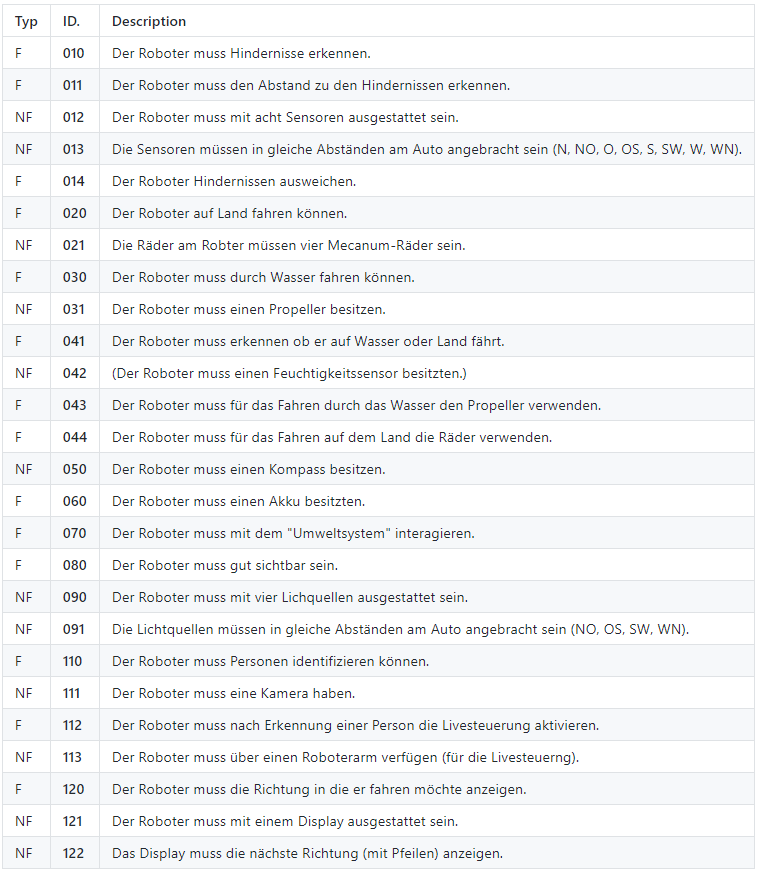
\includegraphics[width=0.5\textwidth]{Bilder/requirements.PNG}
  \caption{Anforderungen}
  \label{fig:anforderungen}
\end{figure}\\
Funktionale Anforderungen (Typ: F) sind Anforderungen die beschreiben was das System oder das Produkt ausführen muss \cite{b1} und nicht-funktionale Anforderungen (Typ: NF) beschreiben die fundamentale Basis der Systemarchitektur \cite{b2}.\\
Das Projekt ist die Simulation eines Rescue Robots.\\
Zusammengefasst sind die Anforderungen folgende: 
\begin{itemize}
    \item Der Roboter muss Hindernisse erkennen und ausweichen.
    \item Der Roboter muss auf Land und Wasser fahren können.
    \item Der Roboter muss seinen Standort weitergeben.
    \item Der Roboter muss anzeigen in welche Richtung er als nächstes fährt.
    \item Der Roboter muss Personen identifizieren.
    \item Der Roboter muss einen Roboterarm besitzen, der per Liveschaltung verwendet wird um Lebewesen und Objekte zu bergen.
\end{itemize}
